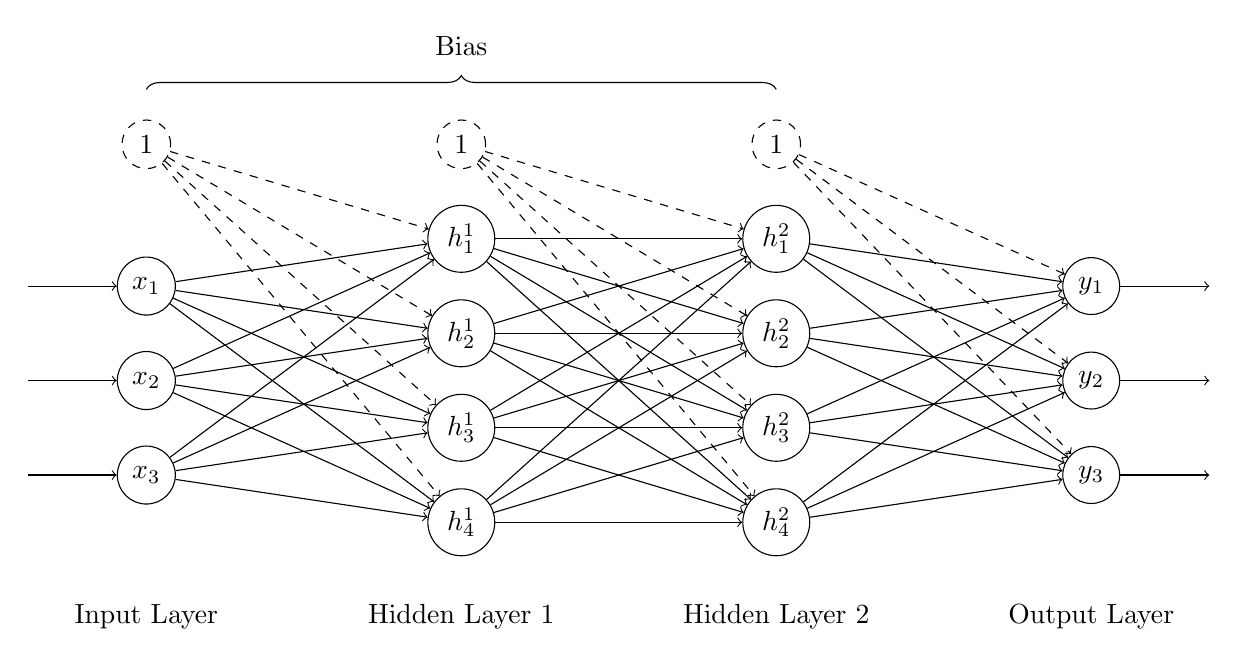
\begin{tikzpicture}
    \tikzstyle{place}=[circle, draw=black, minimum size = 4mm]
    
    % Input
    \draw node [dashed] at (0, 0) [place] (first_0) {$1$};
    \foreach \x in {1,...,3}
      \draw node at (0, -\x*1.2 - 0.6) [place] (first_\x) {$x_\x$};
    \foreach \x in {1,...,3}
      \draw [->] (-1.5, -\x*1.2 - 0.6) to (first_\x); 
    
    % Hidden 1
    \draw node [dashed] at (4, 0) [place] (second_0) {$1$};
    \foreach \x in {1,...,4}
      \node at (4, -\x*1.2) [place] (second_\x) {$h^{1}_\x$};

    % Hidden 2
    \draw node [dashed] at (8, 0) [place] (third_0) {$1$};
    \foreach \x in {1,...,4}
      \node at (8, -\x*1.2) [place] (third_\x) {$h^{2}_\x$};
    
    % Output
    \foreach \x in {1,...,3}
      \node at (12, -\x*1.2 - 0.6) [place] (fourth_\x) {$y_\x$};
    \foreach \x in {1,...,3}
      \draw [->] (fourth_\x) to (13.5, -\x*1.2 - 0.6); 

    \draw [decorate,decoration={brace,amplitude=5pt,raise=-2ex}]
      (0,1) -- (8,1) node[above,midway]{Bias};
      
    % Input -> Hidden 1
    \foreach \i in {1,...,4}
      \draw [->,dashed] (first_0) to (second_\i);
    \foreach \i in {1,...,3}
      \foreach \j in {1,...,4}
        \draw [->] (first_\i) to (second_\j);
    
    % Input -> Hidden 2
    \foreach \i in {1,...,4}
      \draw [->,dashed] (second_0) to (third_\i);
    \foreach \i in {1,...,4}
      \foreach \j in {1,...,4}
        \draw [->] (second_\i) to (third_\j);
    
    % Hidden -> Output
    \foreach \i in {1,...,3}
      \draw [->,dashed] (third_0) to (fourth_\i);
    \foreach \i in {1,...,4}
      \foreach \j in {1,...,3}
        \draw [->] (third_\i) to (fourth_\j);
    
    % Text
    \node at (0, -6) [black, ] {Input Layer};
    \node at (4, -6) [black, ] {Hidden Layer 1};
    \node at (8, -6) [black, ] {Hidden Layer 2};
    \node at (12, -6) [black, ] {Output Layer};
  \end{tikzpicture}